\documentclass{beamer}
 
\usepackage[czech]{babel}
\usepackage{color}
\usepackage[utf8]{inputenc}
\usepackage{graphics}
\usepackage{listings}
\usepackage{xcolor}

\usetheme{Madrid}
\definecolor{UBCblue}{rgb}{0.04706, 0.13725, 0.26667}
\usecolortheme[named=UBCblue]{structure}

\definecolor{codegreen}{rgb}{0,0.6,0}
\definecolor{codegray}{rgb}{0.5,0.5,0.5}
\definecolor{codepurple}{rgb}{0.58,0,0.82}
\definecolor{backcolour}{rgb}{0.95,0.95,0.92}

\lstdefinestyle{mystyle}
{
    backgroundcolor=\color{backcolour},   
    commentstyle=\color{codegreen},
    keywordstyle=\color{magenta},
    numberstyle=\tiny\color{codegray},
    stringstyle=\color{codepurple},
    basicstyle=\ttfamily\footnotesize,
    breakatwhitespace=false,         
    breaklines=true,                 
    keepspaces=true,                 
    numbers=left,                    
    numbersep=3pt,                  
    showspaces=false,                
    showstringspaces=false,
    showtabs=false,                  
    tabsize=2
}

\lstset{style=mystyle}

\title{Hashovací Tabulka}
\author{Andrei Shchapaniak}
\institute{VUT FIT}
\date{\today}
 
\begin{document}

    \frame{\titlepage}
    
    \begin{frame}
        \frametitle{Co je to hashovací tabulka?}
        \begin{figure}
            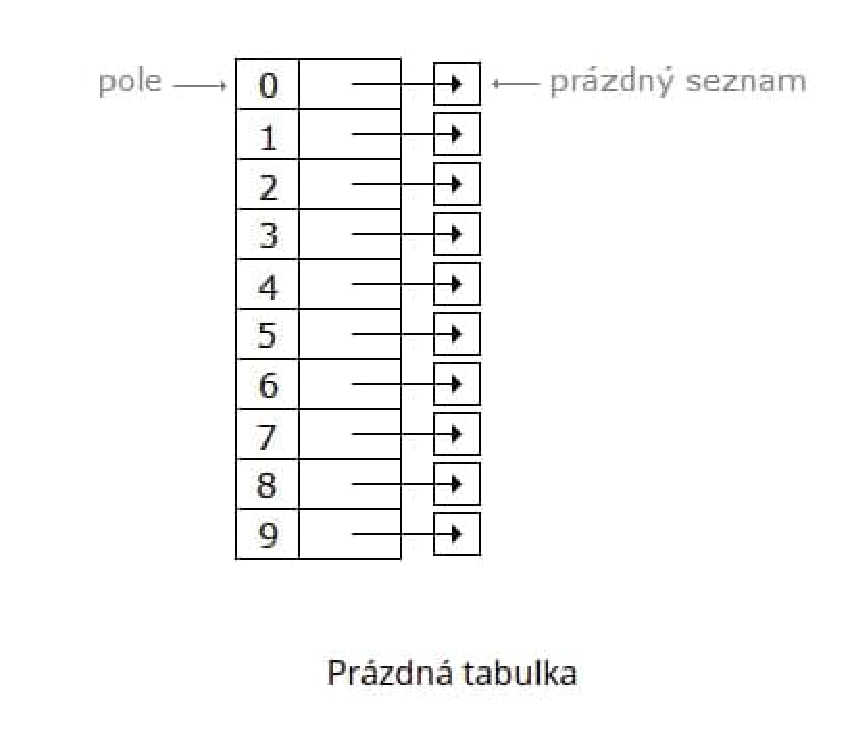
\includegraphics[height=5.0cm]{hash_table.eps}
            \centering
        \end{figure}

        \begin{itemize}
            \item Hashovací tabulka je vyhledávací datová struktura, která asociuje hašovací klíče s odpovídajícími hodnotami.
        \end{itemize}
    \end{frame}

    \begin{frame}
        \frametitle{Kde se používá?}
        \begin{itemize}
            \item Implementace tabulky symbolů v překladači nějakého jazyka
            \item Indexování databáze
            \item Asociativní pole
            \item Objektová reprezentace
            \item Bezpečné třídění IP adres
        \end{itemize}
    \end{frame}

    \begin{frame}[fragile]{Inicializace struktur hashovací tabulky}
        \begin{lstlisting}[language=C]
    // // Define the Hash Table Item here
    typedef struct Ht_item {
        char* key;
        char* value;
    } Ht_item;
    
    // Define the Hash Table here
    define struct HashTable {
        // Contains an array of pointers
        // to items
        Ht_item** items;
        int size;
        int count;
    } HashTable;
        \end{lstlisting}
    \end{frame}
    
    \begin{frame}[fragile]{Inicializace prvku hashovací tabulky}
        \begin{lstlisting}[language=C]
    Ht_item* create_item(char* key, char* value) {
        // Creates a pointer to a new hash table item
        Ht_item* item = (Ht_item*) malloc (sizeof(Ht_item));
        
        item->key = (char*) malloc (strlen(key) + 1);
        item->value = (char*) malloc (strlen(value) + 1);
        
        strcpy(item->key, key);
        strcpy(item->value, value);
        
        return item;
    }
        \end{lstlisting}
    \end{frame}
    
    \begin{frame}[fragile]{Inicializace hashovací tabulky}
        \begin{lstlisting}[language=C]
    HashTable* create_table(int size) {
        // Creates a new HashTable
        HashTable* table = (HashTable* )malloc (sizeof(HashTable));
        
        table->size = size;
        table->count = 0;
        
        table->items = (Ht_item**) calloc (table->size, sizeof(Ht_item*));
        
        for (int i=0; i<table->size; i++)
            table->items[i] = NULL;
            
        return table;
    }
        \end{lstlisting}
    \end{frame}
    
    \begin{frame}[fragile]{Vyčištění alokované pamětí}
        \begin{lstlisting}[language=C]
    void free_item(Ht_item* item) {
        // Frees an item
        free(item->key);
        free(item->value);
        free(item);
    }
     
    void free_table(HashTable* table) {
        // Frees the table
        for (int i=0; i<table->size; i++) {
            Ht_item* item = table->items[i];
            if (item != NULL)
                free_item(item);
        }
     
        free(table->items);
        free(table);
    }
        \end{lstlisting}
    \end{frame}
    
    \begin{frame}
        \frametitle{Výhody a nevýhody hashovací tabulky}
        \begin{itemize}
            \item Hashovací tabulka je velmi efektivní vyhledávací metoda
            \item Pokud uvažujeme ideální případ, hashovací tabulka je rychkejší než binární vyhledávací strom
            \item Neposkytuje intervalové dotazy, tj. vyhledání všech klíčů v daném intervalu
            \item Hašovací tabulka umožňuje pouze dotazy na jednotlivé klíče
        \end{itemize}
    \end{frame}
    
    \begin{frame}
        \frametitle{Zdroje}
        \begin{itemize}
            \item Wikipedie \href{https://cz.wikipedia.org/wiki/Hash_table}{\beamergotobutton{Link}}
            \item Práce s hashovací tabulkou \href{https://www.itnetwork.cz/navrh/algoritmy/algoritmy-vyhledavani/algoritmus-vyhledavani-hashovaci-tabulka}{\beamergotobutton{Link}}
            \item Kod \href{https://www.journaldev.com/35238/hash-table-in-c-plus-plus}{\beamergotobutton{Link}}
        \end{itemize}
    \end{frame}
    
\end{document}
